% TEX compiler = luatex
% copyright arturo salinas-aguayo 2025
\documentclass[12pt]{article}

\usepackage{graphicx}
\usepackage{amsmath}
\usepackage{array}
\usepackage{amsfonts}
\usepackage{fancyhdr}
\usepackage{geometry}
\usepackage{circuitikz}
\usepackage{subfigure}
\usepackage{caption}
\usepackage{karnaugh-map}
\usepackage{bm}
\usepackage{float}

\geometry{letterpaper, margin=1in}
\graphicspath{ {../../images/} }

% Header and Footer
\pagestyle{fancy}
\fancyhf{}
\fancyhead[L]{ECE 2001 - Lab 05: First-Order Circuits}
\fancyhead[R]{\thepage}
\setlength{\headheight}{15pt}

\author{Arturo Salinas-Aguayo}
\title{Lab 05: First-Order Circuits}

% theorem set
\newtheorem{example}{Example}
% Example block environment
\newenvironment{examp}
{\vspace{0.5cm}
 \hrule
\vspace{0.5cm}
\begin{example}}
{\hrule
\vspace{0.5cm}
\end{example}}

\begin{document}
\newcommand{\closure}[2][3]{%
	{}\mkern#1mu\overline{\mkern-#1mu#2}}
\newcommand\ncoverline[1]{\mkern1mu\overline{\mkern-1mu#1\mkern-1mu}\mkern1mu}
% Title Page
\begin{titlepage}
	\centering
	\vspace*{3cm}
	\huge\textbf{Lab 05: First-Order Circuits}\\

	\vspace{5cm}
	\Large\textbf{Arturo Salinas-Aguayo}\\
	\normalsize
	ECE 2001 Electrical Circuits\\
	Dr. David J. Giblin, Section 331.660.701.810-1253\\
	Mechanical Engineering Department
	\vfill
	
\includegraphics[scale=0.1]{uconnlogo}\\
	College of Engineering, University of Connecticut\\
	\scriptsize{Coded in \LaTeX}
	\vspace*{1cm}
\end{titlepage}
\tableofcontents
\newpage
\section{Abstract}
\newpage
\section{Introduction}
\section{Theory}
\section{Experimental Procedures}
\subsection{Circuit One}
Initial voltage $V_0 = 0V$, Resistance $R = 10M\Omega$, Capacitance $C = 10\mu F$, Final voltage $V_f = 10V$.

The time constant $\tau = RC = 10M\Omega \times 10\mu F = 100s$.

Transient response:
\[
	v_C(t) = V_f (1 - e^{-\frac{t}{\tau}})
\]
\[
	v_C(t) = 10V (1 - e^{-\frac{t}{100s}})
\]
\begin{figure}[H]
	\centering
	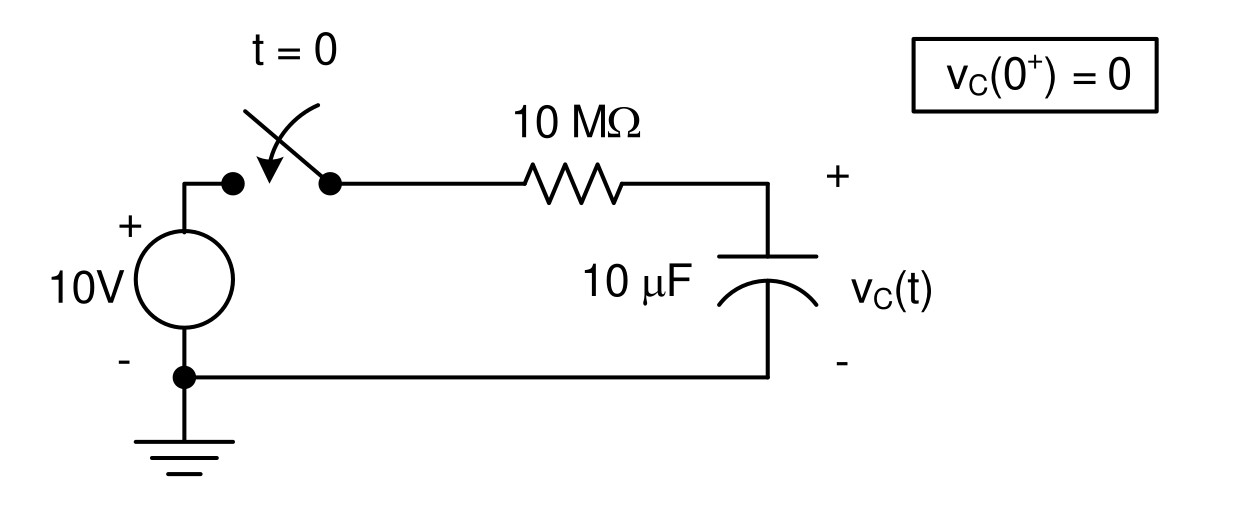
\includegraphics[width=14cm]{e5_1}
	\caption{An Virgin Resistive Capacitive Circuit}
\end{figure}
\subsection{Circuit Two}
Initial voltage $V_0 = 10V$, Resistance $R = 10M\Omega$, Capacitance $C = 10\mu F$, Final voltage $V_f = 0V$.

The time constant $\tau = RC = 10M\Omega \times 10\mu F = 100s$.

Transient response:
\[
	v_C(t) = V_0 e^{-\frac{t}{\tau}}
\]
\[
	v_C(t) = 10V e^{-\frac{t}{100s}}
\]
\begin{figure}[H]
	\centering
	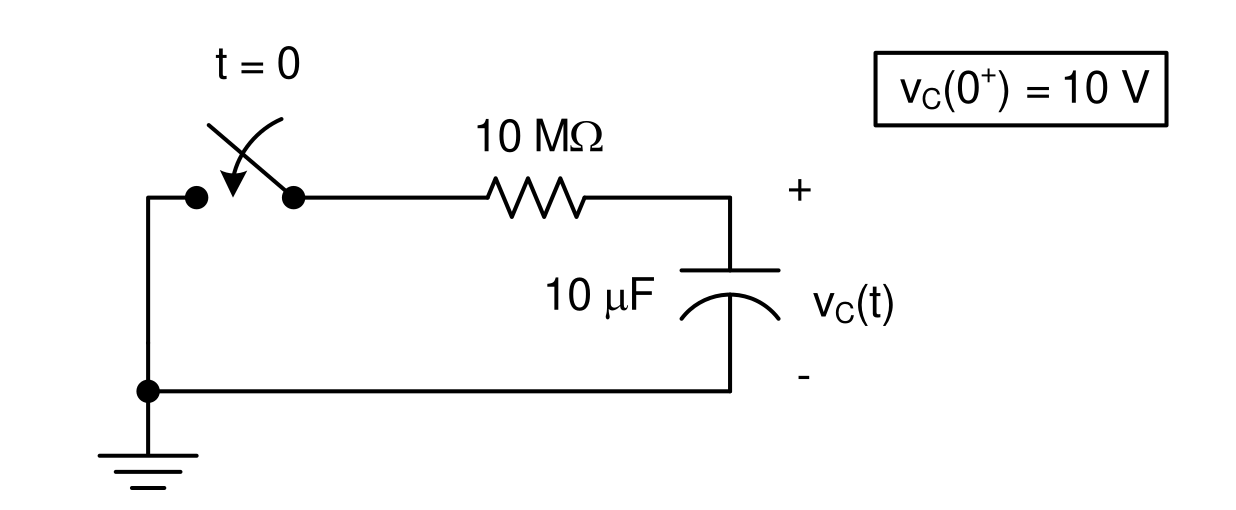
\includegraphics[width=14cm]{e5_2}
	\caption{An Excited Resistive Capacitive Circuit}
\end{figure}
\subsection{Circuit Three}
Resistance $R = 2.0k\Omega$, Capacitance $C = 10nF$, Time Constant $\tau = 20\mu s$.

Transient response for a square wave input with $5V$ amplitude and $T = 200\mu s$:
\[
	v_C(t) = 5V(1 - e^{-\frac{t}{20\mu s}}) \quad \text{during charging}
\]
\[
	v_C(t) = 5V e^{-\frac{t}{20\mu s}} \quad \text{during discharging}
\]
$V_c(0^+) = 0V$
The Time Constant, $\tau$ is calculated for this circuit.
\begin{align*}
	\tau & = RC = 10nF * 2.0k\Omega \\
	\tau & = 20\mu s
\end{align*}
The time constant is then multiplied by a factor of ten to obtain the period for
the input sine wave.
\begin{align*}
	\tau \cdot 10 & = T        \\
	20\mu s * 10  & = 200\mu s \\
\end{align*}
\begin{figure}[H]
	\centering
	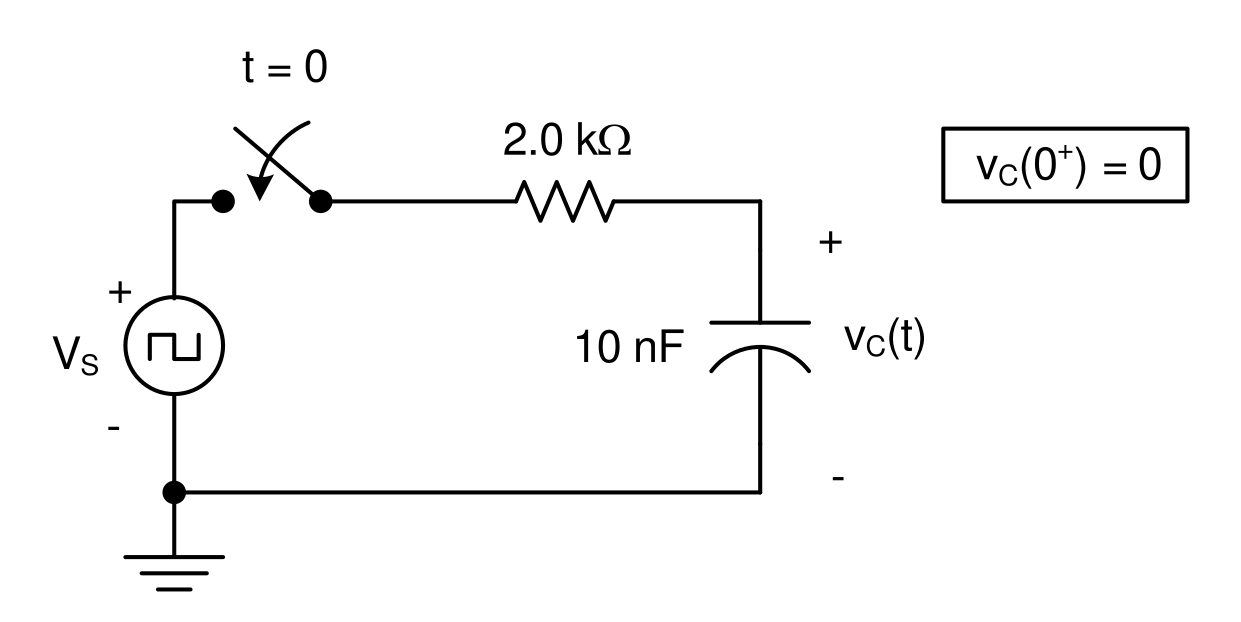
\includegraphics[width=14cm]{e5_3}
	\caption{A Square Wave Input RC Circuit}
\end{figure}
\subsection{Circuit Four}
Resistance $R = 100k\Omega$, Capacitance $C = 100pF$, Time Constant $\tau = 10\mu s$.

Transient response for a square wave input with $5V$ amplitude and $T = 100\mu s$:
\[
	v_C(t) = 5V(1 - e^{-\frac{t}{10\mu s}}) \quad \text{during charging}
\]
\[
	v_C(t) = 5V e^{-\frac{t}{10\mu s}} \quad \text{during discharging}
\]
$V_c(0^+) = 0V$
The Time Constant, $\tau$ is calculated for this circuit.
\begin{align*}
	\tau & = RC = 100pF * 100.0k\Omega \\
	\tau & = 10\mu s
\end{align*}
The time constant is then multiplied by a factor of ten to obtain the period for
the input sine wave.
\begin{align*}
	\tau \cdot 10 & = T        \\
	10\mu s * 10  & = 100\mu s \\
\end{align*}
\begin{figure}[H]
	\centering
	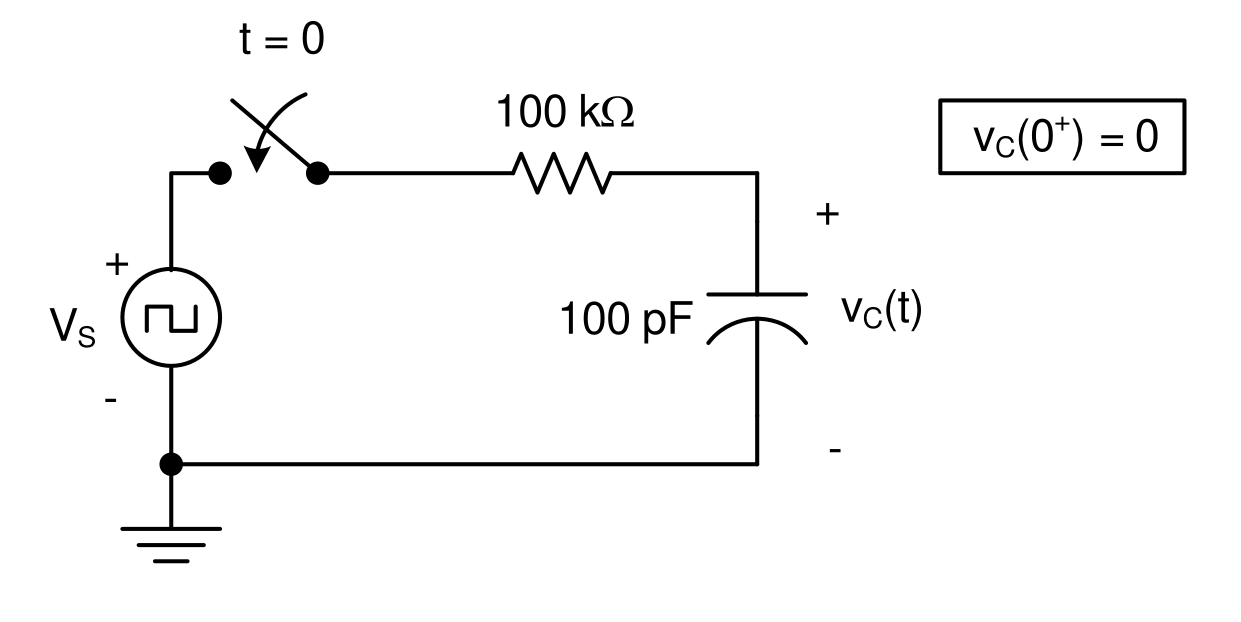
\includegraphics[width=14cm]{e5_4}
	\caption{Circuit Three with Adjusted Components}
\end{figure}
\subsection{Circuit Five}
Inductance $L = 10mH$, Resistance $R = 100\Omega$, Time Constant $\tau = 100\mu s$.

Transient response for a square wave input with $1V$ amplitude and $T = 1.0 ms$:
\[
	i_L(t) = \frac{V}{R}(1 - e^{-\frac{t}{\tau}}) \quad \text{during the positive half-cycle}
\]
\[
	i_L(t) = \frac{V}{R} e^{-\frac{t}{\tau}} \quad \text{during the negative half-cycle}
\]

$I_L(0^+) = 0A$
The Time Constant, $\tau$ is calculated for this circuit.
\begin{align*}
	\tau & = \frac{L}{R} = \frac{10mH}{100\Omega} \\
	\tau & = 100\mu s
\end{align*}
The time constant is then multiplied by a factor of ten to obtain the period for
the input sine wave.
\begin{align*}
	\tau \cdot 10 & = T      \\
	100\mu s * 10 & = 1.0 ms \\
\end{align*}
\begin{figure}[H]
	\centering
	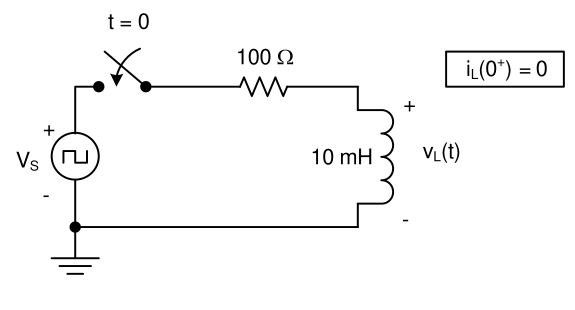
\includegraphics[width=14cm]{e5_5}
	\caption{A Resistive-Inductive Circuit with Square Wave}
\end{figure}
\section{Results and Discussion}
\subsection{Circuit One: Charging Transient}
Measure the transient response for the RC circuit (Figure 5-1) as described.

\subsubsection{Data Table for Circuit One}
\begin{tabular}{ccc}
	\toprule
	Time (s) & Voltage (V) & Notes                          \\
	\midrule
	0        & 0           & Capacitor initially discharged \\
	% Add more rows as necessary
	\bottomrule
\end{tabular}

\subsubsection{Analysis}
\textbf{Question:} Are the final voltage and the time constant within the expected variations due to tolerances?

\textbf{Answer:} \\
% Space for answer

\subsection{Circuit Two: Discharging Transient}
Measure the discharge transient for the RC circuit (Figure 5-2).

\subsubsection{Data Table for Circuit Two}
\begin{tabular}{ccc}
	\toprule
	Time (s) & Voltage (V) & Notes                   \\
	\midrule
	0        & 10          & Capacitor fully charged \\
	% Add more rows as necessary
	\bottomrule
\end{tabular}

\subsubsection{Analysis}
\textbf{Question:} Estimate the time constant from your data. Is this result expected?

\textbf{Answer:} \\
% Space for answer

\subsection{Circuit Three: Response to a Square Wave}
Measure the transient response using a square wave input (Figure 5-3).

\subsubsection{Oscilloscope Image}
\begin{figure}[H]
	\centering
	\includegraphics[width=10cm]{oscilloscope_5_3.png}
	\caption{Oscilloscope display for Circuit Three}
\end{figure}

\subsubsection{Analysis}
\textbf{Question:} Does the experimental time constant agree with your calculations and PSpice analysis?

\textbf{Answer:} \\
% Space for answer

\subsection{Circuit Four: Square Wave Response}
Repeat the measurement for Circuit Four with adjusted component values.

\subsubsection{Oscilloscope Image}
\begin{figure}[H]
	\centering
	\includegraphics[width=10cm]{oscilloscope_5_4.png}
	\caption{Oscilloscope display for Circuit Four}
\end{figure}

\subsubsection{Analysis}
\textbf{Question:} Does the experimental time constant match the calculated value?

\textbf{Answer:} \\
% Space for answer

\subsection{Circuit Five: RL Circuit Response}
Measure the transient response for the RL circuit (Figure 5-5) using a square wave.

\subsubsection{Oscilloscope Image}
\begin{figure}[H]
	\centering
	\includegraphics[width=10cm]{oscilloscope_5_5.png}
	\caption{Oscilloscope display for Circuit Five}
\end{figure}

\subsubsection{Analysis}
\textbf{Question:} Is the transient response as expected? How does the experimental setup affect the results?

\textbf{Answer:} \\
% Space for answer

\section{Conclusion}
\end{document}
% vim: set ft=tex tw=80 ts=2 sts=2 sw=2 noet spell:
